\documentclass[10pt, letterpaper]{article}
\usepackage{lmodern}
% Packages:
\usepackage[
    ignoreheadfoot, % set margins without considering header and footer
    top=2 cm, % seperation between body and page edge from the top
    bottom=2 cm, % seperation between body and page edge from the bottom
    left=2 cm, % seperation between body and page edge from the left
    right=2 cm, % seperation between body and page edge from the right
    footskip=1.0 cm, % seperation between body and footer
    % showframe % for debugging 
]{geometry} % for adjusting page geometry
\usepackage{titlesec} % for customizing section titles
\usepackage{tabularx} % for making tables with fixed width columns
\usepackage{array} % tabularx requires this
\usepackage[dvipsnames]{xcolor} % for coloring text
\definecolor{primaryColor}{RGB}{54, 91, 122}
\definecolor{sectioncolor}{RGB}{96, 63, 44}
\definecolor{linecolor}{RGB}{118, 82, 59}
\definecolor{synblue}{RGB}{58, 107, 176}
\definecolor{manorange}{RGB}{222, 133, 48}
\definecolor{dexteal}{RGB}{41, 140, 133}
\definecolor{paperfill}{RGB}{249, 244, 238}
\definecolor{panelborder}{RGB}{205, 189, 176}
\usepackage{enumitem} % for customizing lists
\usepackage{fontawesome5} % for using icons
\usepackage{amsmath} % for math
\usepackage{graphicx}
\usepackage[
    pdftitle={Yanming Shao's CV},
    pdfauthor={Yanming Shao},
    pdfcreator={LaTeX with RenderCV},
    colorlinks=true,
    urlcolor=blue
]{hyperref}
\hypersetup{
  colorlinks=true,
  urlcolor=primaryColor,
  linkcolor=primaryColor,
  citecolor=primaryColor
}

\usepackage[pscoord]{eso-pic} % for floating text on the page
\usepackage{calc} % for calculating lengths
\usepackage{bookmark} % for bookmarks
\usepackage{lastpage} % for getting the total number of pages
\usepackage{changepage} % for one column entries (adjustwidth environment)
\usepackage{paracol} % for two and three column entries
\usepackage{ifthen} % for conditional statements
\usepackage{needspace} % for avoiding page brake right after the section title
\usepackage{iftex} % check if engine is pdflatex, xetex or luatex

% Ensure that generate pdf is machine readable/ATS parsable:
\ifPDFTeX
    \input{glyphtounicode}
    \pdfgentounicode=1
    % \usepackage[T1]{fontenc} % this breaks sb2nov
    \usepackage[utf8]{inputenc}
    \usepackage{lmodern}
\fi



% Some settings:
\AtBeginEnvironment{adjustwidth}{\partopsep0pt} % remove space before adjustwidth environment
\pagestyle{empty} % no header or footer
\setcounter{secnumdepth}{0} % no section numbering
\setlength{\parindent}{0pt} % no indentation
\setlength{\topskip}{0pt} % no top skip
\setlength{\columnsep}{0cm} % set column seperation
\makeatletter
\let\ps@customFooterStyle\ps@plain % Copy the plain style to customFooterStyle
\patchcmd{\ps@customFooterStyle}{\thepage}{
    \color{gray}\textit{\small Yanming Shao - Page \thepage{} of \pageref*{LastPage}}
}{}{} % replace number by desired string
\makeatother
\pagestyle{customFooterStyle}



\titleformat{\section}
  {\needspace{4\baselineskip}\bfseries\large\color{sectioncolor}} % apply color to title text
  {}{0pt}{} % keep label and spacing as before
  [\vspace{1pt}{\color{sectioncolor}\titlerule}]   % color the rule


\titlespacing{\section}{
    % left space:
    -1pt
}{
    % top space:
    0.22 cm
}{
    % bottom space:
    0.16 cm
} % section title spacing

\renewcommand\labelitemi{$\circ$} % custom bullet points
\newenvironment{highlights}{
    \begin{itemize}[
        topsep=0.10 cm,
        parsep=0.10 cm,
        partopsep=0pt,
        itemsep=0pt,
        leftmargin=0.4 cm + 10pt
    ]
}{
    \end{itemize}
} % new environment for highlights

\newenvironment{highlightsforbulletentries}{
    \begin{itemize}[
        topsep=0.10 cm,
        parsep=0.10 cm,
        partopsep=0pt,
        itemsep=0pt,
        leftmargin=10pt
    ]
}{
    \end{itemize}
} % new environment for highlights for bullet entries

\setlist[enumerate]{
    leftmargin=*,
    itemsep=0.04 cm,
    topsep=0.06 cm,
    parsep=0pt,
    partopsep=0pt
}

\setlist[itemize]{
    itemsep=0.02 cm,
    topsep=0.06 cm,
    parsep=0pt,
    partopsep=0pt
}

% Defines the rSection environment for the large sections within the CV

\usepackage{xspace}
\newcommand{\synpoldex}{\textbf{SynPolDex}\xspace}
\newcommand{\bimangrasp}{\textbf{BimanGrasp}\xspace}
\newcommand{\SynManDexName}{\textcolor{synblue}{\textbf{Syn}}\textcolor{manorange}{\textbf{Man}}\textcolor{dexteal}{\textbf{Dex}}}

\newenvironment{onecolentry}{
    \begin{adjustwidth}{
        0.2 cm + 0.00001 cm
    }{
        0.2 cm + 0.00001 cm
    }
}{
    \end{adjustwidth}
} % new environment for one column entries

\newenvironment{twocolentry}[2][]{
    \onecolentry
    \def\secondColumn{#2}
    \setcolumnwidth{\fill, 4.5 cm}
    \begin{paracol}{2}
}{
    \switchcolumn \raggedleft \secondColumn
    \end{paracol}
    \endonecolentry
} % new environment for two column entries

\newenvironment{header}{
    \setlength{\topsep}{0pt}\par\kern\topsep\centering\linespread{1.42}
}{
    \par\kern\topsep
} % new environment for the header

\newcommand{\placelastupdatedtext}{% \placetextbox{<horizontal pos>}{<vertical pos>}{<stuff>}
  \AddToShipoutPictureFG*{% Add <stuff> to current page foreground
    \put(
        \LenToUnit{\paperwidth-2 cm-0.2 cm+0.05cm},
        \LenToUnit{\paperheight-1.0 cm}
    ){\vtop{{\null}\makebox[0pt][c]{
        \small\color{gray}\textit{Last updated in March 2026}\hspace{\widthof{Last updated in March 2026}}
    }}}%
  }%
}%

% save the original href command in a new command:
\let\hrefWithoutArrow\href

% new command for external links:
\renewcommand{\href}[2]{\hrefWithoutArrow{#1}{\ifthenelse{\equal{#2}{}}{ }{#2 }\raisebox{.15ex}{\footnotesize \faExternalLink*}}}

\newcommand{\SynPolDex}{\textbf{SynPolDex}\xspace}
\newcommand{\BimanGrasp}{\textbf{BimanGrasp}\xspace}

\begin{document}
    \newcommand{\AND}{\unskip
        \cleaders\copy\ANDbox\hskip\wd\ANDbox
        \ignorespaces
    }
    \newsavebox\ANDbox
    \sbox\ANDbox{}

    \placelastupdatedtext
    \begin{header}
        \textbf{\fontsize{24 pt}{24 pt}\selectfont YANMING SHAO}

        \vspace{0.24 cm}

        \normalsize
        \mbox{{\color{black}\footnotesize\faMapMarker*}\hspace*{0.13cm}ShanghaiTech University, 1 Zhongke Road, Pudong 201210, Shanghai}%
        \kern 0.25 cm%
        \AND%
        \kern 0.25 cm%
        \mbox{\hrefWithoutArrow{mailto:shaoyanming@pjlab.org.cn}{\color{black}{\footnotesize\faEnvelope[regular]}\hspace*{0.13cm}shaoyanming@pjlab.org.cn}}%
        \kern 0.25 cm%
        \AND%
        \kern 0.25 cm%
        \mbox{\hrefWithoutArrow{mailto:shaoym2023@shanghaitech.edu.cn}{\color{black}{\footnotesize\faEnvelope[regular]}\hspace*{0.13cm}shaoym2023@shanghaitech.edu.cn}}%
        \kern 0.25 cm%
        \AND%
        \kern 0.25 cm%
        \mbox{\hrefWithoutArrow{tel:+86-180-1906-7367}{\color{black}{\footnotesize\faPhone*}\hspace*{0.13cm}+86-180-1906-7367}}%
        
        \vspace{0.09 cm}

        \mbox{\hrefWithoutArrow{https://tsunami-kun.github.io/}{\color{blue}{\footnotesize\faLink}\hspace*{0.13cm}Homepage}}%
        \kern 0.25 cm%
        \AND%
        \mbox{\hrefWithoutArrow{https://scholar.google.com/citations?user=gHy232gAAAAJ&hl=en}{\color{blue}{\footnotesize\faGoogle}\hspace*{0.13cm}Google Scholar}}%
        \kern 0.25 cm%
        \AND%
        \kern 0.25 cm%
        \mbox{\hrefWithoutArrow{https://github.com/Tsunami-kun}{\color{blue}{\footnotesize\faGithub}\hspace*{0.13cm}Github}}%
    \end{header}

    \vspace{0.3 cm - 0.3 cm}


\section{RESEARCH INTERESTS}


\textbf{Bimanual Dexterous Manipulation}
\begin{onecolentry}
    \begin{highlightsforbulletentries}
    \item Developing human-like dexterous manipulation for embodied AI systems, especially beyond two-fingered grippers, including in-hand rotation and multi-object grasping.
    \end{highlightsforbulletentries}
\end{onecolentry}

\textbf{Scaling Robotic Data}
\begin{onecolentry}
    \begin{highlightsforbulletentries}
    \item Studying how robotic data scales across embodiments, sensors, and task diversity, with emphasis on video, force, and tactile data for general-purpose manipulation models.
    \end{highlightsforbulletentries}
\end{onecolentry}


% \href{https://docs.rendercv.com/user_guide/}{Here}



    
\section{PUBLICATIONS}

\textbf{Major Contributions}

\begin{enumerate}[label={[\arabic*]}]
  \item \textbf{Yanming Shao} and Chenxi Xiao*, 
        ``Bimanual Grasp Synthesis for Dexterous Robot Hands,'' 
        \emph{IEEE Robotics and Automation Letters}, Nov. 2024. \hrefWithoutArrow{https://bimangrasp.github.io/}{(Project Page)} 
        \hrefWithoutArrow{https://bimangrasp.github.io/static/pdfs/paper.pdf/}{(PDF)}
        \hrefWithoutArrow{https://github.com/Tsunami-kun/BimanGrasp-Dataset/}{(Dataset)}  \hrefWithoutArrow{https://bimangrasp.github.io/static/video/BimanGrasp.mp4/}{(Video)}
        
  \item \textbf{Yanming Shao}, Yan Ding*, and Chenxi Xiao*, 
        ``SynPolDex: Synergizing Fingers via Bi-Level Policy Learning for Dexterous Robotic Hands,'' 
        \emph{2025 IEEE-RAS 24th International Conference on Humanoid Robots (Humanoids)}, 2025.

  \item \textbf{Yanming Shao}, et al.,
        ``SynManDex: Human-like Dexterous Grasping from Synthetic Human Priors,''
        \emph{in submission}, 2026.
\end{enumerate}

\textbf{Collaborative Papers}

\begin{enumerate}[label={[\arabic*]}, resume]
  \item Yifan Han, Zhongxi Chen, Yuxuan Zhao, Congsheng Xu, \textbf{Yanming Shao}, Yichuan Peng, Yao Mark Mu, and Wenzhao Lian,
        ``DexHiL: A Human-in-the-Loop Framework for Vision-Language-Action Model Post-Training in Dexterous Manipulation,''
        \emph{arXiv preprint arXiv:2603.09121}, 2026. \hrefWithoutArrow{https://arxiv.org/abs/2603.09121}{(arXiv)}

  \item Yiteng Chen, Zhe Cao, Hongjia Ren, Chenjie Yang, Wenbo Li, Shiyi Wang, Yemin Wang, Li Zhang, \textbf{Yanming Shao}, Zhenjun Zhao, Huiping Zhuang, and Qingyao Wu,
        ``RoboRouter: Training-Free Policy Routing for Robotic Manipulation,''
        \emph{arXiv preprint arXiv:2603.07892}, 2026. \hrefWithoutArrow{https://arxiv.org/abs/2603.07892}{(arXiv)}
\end{enumerate}

\textbf{In Submission}

\begin{enumerate}[label={[\arabic*]}, resume]
  \item Bin Qiu, \textbf{Yanming Shao}, Guanyu Cai, and Yao Mark Mu,
        ``Enforcing Human-like Kinematics in Dexterous Piano Playing via Adversarial Posture Regularization.''

  \item Kaihan Chen, \textbf{Yanming Shao}, Haifeng Ji, Xiaokang Yang, and Yao Mark Mu,
        ``V2P-Manip: Learning Single-hand Dexterous Manipulation from Monocular Human Videos.''
\end{enumerate}

% \href{https://doi.org/10.1109/TASC.2023.3340648}{10.1109/TASC.2023.3340648}

\section{EDUCATION}

    \begin{twocolentry}{ 
    \textit{Sept 2023 – May 2026 (expected)}}
        \textbf{Master, ShanghaiTech University}
        
        \textit{Academic Master's Student of Engineering, Major in Computer Science}
    \end{twocolentry}

    \begin{twocolentry}{ 
    \textit{Sept 2017 – May 2022}}
        \textbf{Bachelor, ShanghaiTech University}
        
        \textit{B.E. of Engineering, Major in Electric Engineering}
    \end{twocolentry}


\section{RESEARCH EXPERIENCES}

    \begin{twocolentry}{
    \textit{}    
        
    \textit{Sep 2023 – Present}}
        \textbf{Graduate Research Assistant}
        
        \textit{RIM Lab, ShanghaiTech University \hfill (with Chenxi Xiao)}
    \end{twocolentry}

    \vspace{0.08 cm}

    \begin{twocolentry}{
    \textit{}    
        
    \textit{Nov 2024 – March 2025}}
        \textbf{Research Intern}
        
        \textit{IPEC, Shanghai AI Laboratory \hfill (with Yan Ding)}
    \end{twocolentry}

    \vspace{0.08 cm}

    \begin{twocolentry}{
    \textit{}

    \textit{June 2025 – Oct 2025}}
        \textbf{Research Intern}
        
        \textit{Shanghai Qizhi Institute \hfill (with Macheng Shen)}
    \end{twocolentry}

    \vspace{0.08 cm}

    \begin{twocolentry}{
    \textit{}

    \textit{Oct 2025 – Present}}
        \textbf{Research Intern}
        
        \textit{Intern Robotics, Shanghai AI Laboratory \hfill (with Yao Mark Mu)}
    \end{twocolentry}


\newpage



\section{FEATURED PROJECT}

\begin{twocolentry}{
\textit{}    
    
\textit{2025 – Present}}
\textbf{\SynManDexName}: Human-like Dexterous Grasping from Synthetic Human Priors
    
    \textit{Lead project at ShanghaiTech RIM Lab on human-like dexterous grasp synthesis, synthetic demonstration generation, and bimanual manipulation policy learning.}

    \textit{ }
\end{twocolentry}

\vspace{0.04 cm}

\begin{onecolentry}
\setlength{\fboxsep}{8pt}
\fcolorbox{panelborder}{paperfill}{
\parbox{0.965\linewidth}{
\linespread{1.04}\selectfont
\textit{\SynManDexName{} unifies human-likeness and physical correctness for dexterous grasping. The pipeline first samples human pre-grasps from object geometry with a conditional diffusion model, retargets them to multi-fingered robot hands, refines them with force-closure optimization regularized by human priors, and then converts validated grasps into full arm-hand trajectories for policy learning.}
}
}
\end{onecolentry}

\vspace{0.05 cm}

\begin{onecolentry}
    \begin{highlightsforbulletentries}
        \item \textbf{SynManDex-Human}: a conditional diffusion model that synthesizes diverse human pre-grasps from object geometry alone.
        \item \textbf{SynManDex-Optimization}: position-based retargeting plus force-closure refinement, preserving human-like structure while enforcing stable contacts.
        \item \textbf{SynManDex-ACT}: a unified 36-DoF bimanual policy trained on generated demonstrations, reaching \textbf{71.4\%} grasp-and-lift success and nearly doubling the optimization-only baseline (\textbf{37.1\%}).
    \end{highlightsforbulletentries}
\end{onecolentry}

\vspace{0.03 cm}

\begin{onecolentry}
\centering
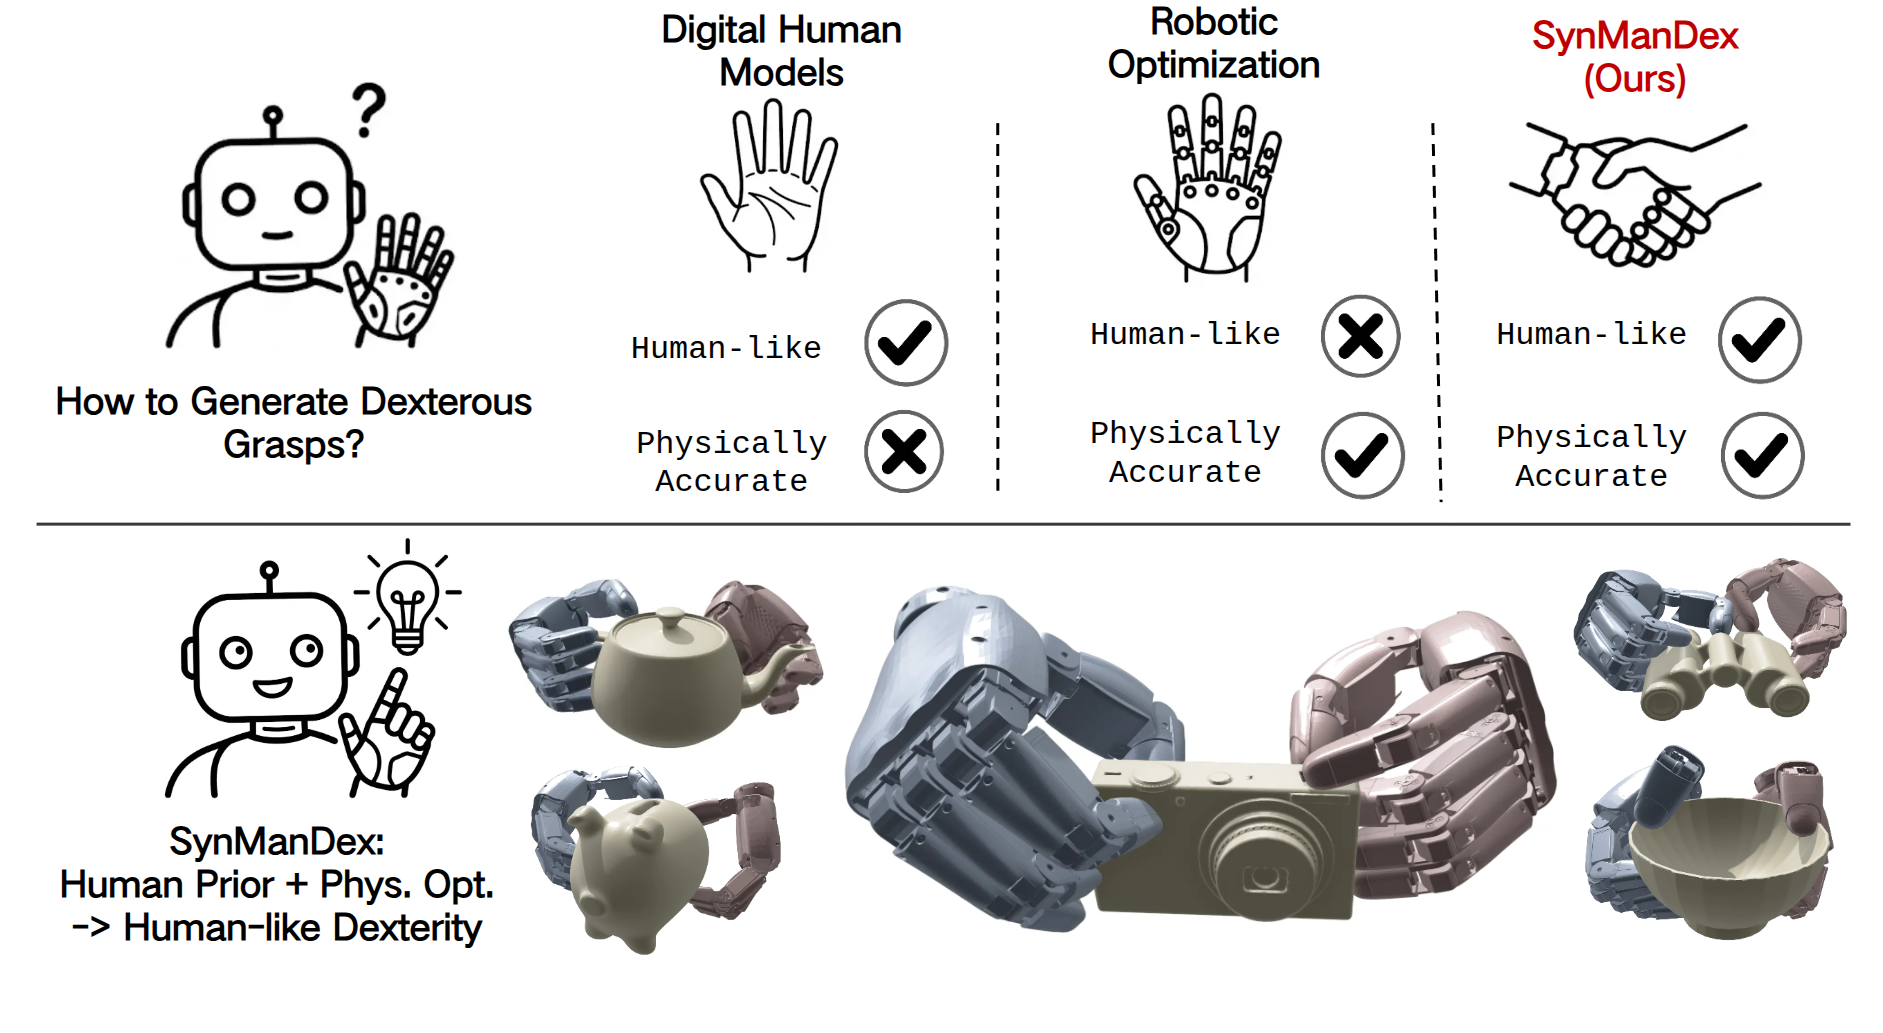
\includegraphics[width=.92\linewidth]{img/synmandex_teaser.png}

\vspace{0.14 cm}
{\small \linespread{1.03}\selectfont \textbf{\SynManDexName{} at a glance.} Human priors provide natural pre-grasps, physics-based refinement makes them valid for robot hands, and the resulting trajectories support contact-rich bimanual policy learning.\par}

\vspace{0.28 cm}
\begin{minipage}[t]{0.54\linewidth}
    \centering
    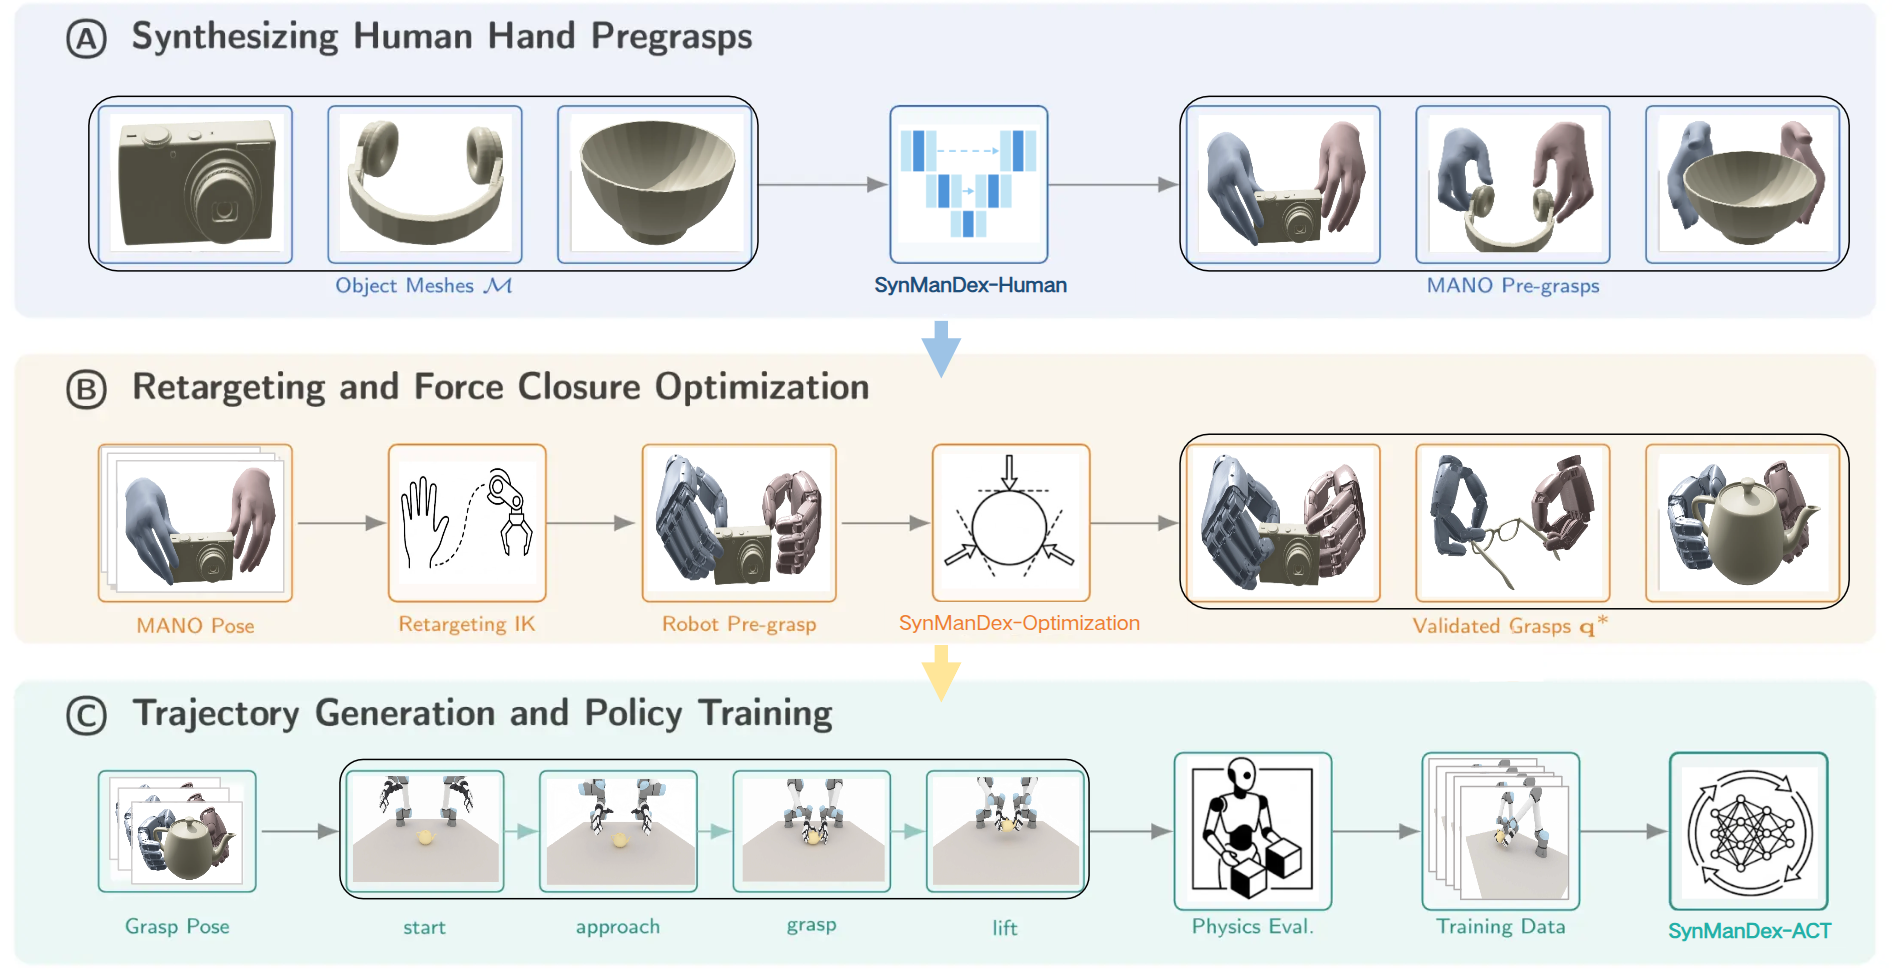
\includegraphics[width=\linewidth]{img/synmandex_system.png}

    \vspace{0.13 cm}
    {\small \linespread{1.03}\selectfont Three-stage pipeline: pre-grasp diffusion, robot-hand refinement, and geometry-consistent trajectory generation.\par}
\end{minipage}
\hfill
\begin{minipage}[t]{0.42\linewidth}
    \centering
    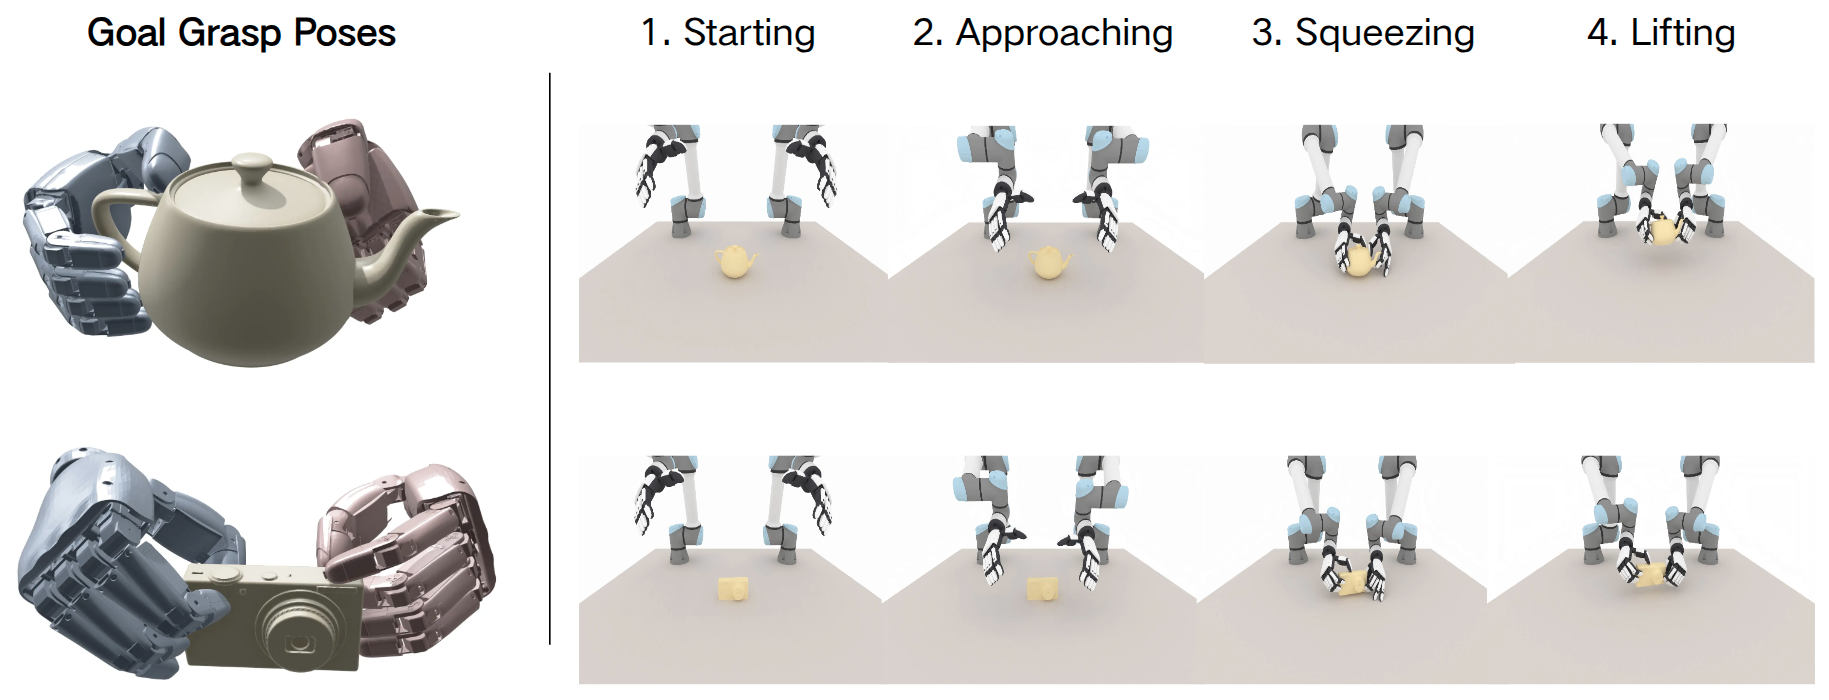
\includegraphics[width=\linewidth]{img/synmandex_traj.png}

    \vspace{0.13 cm}
    {\small \linespread{1.03}\selectfont Qualitative trajectories preserve human-like contact semantics while remaining executable on a 36-DoF bimanual platform.\par}
\end{minipage}
\end{onecolentry}

\newpage

\section{RESEARCH PROJECTS}

\begin{twocolentry}{
\textit{}    
    
\textit{2024}}
\textbf{BimanGrasp}
    
    \textit{Project at ShanghaiTech RIM Lab. We proposed the BimanGrasp pipeline and built a large-scale bimanual dexterous grasp dataset over 900 daily objects.}

    \textit{ }
\end{twocolentry}

\begin{figure*}[htpb]
    \centering
    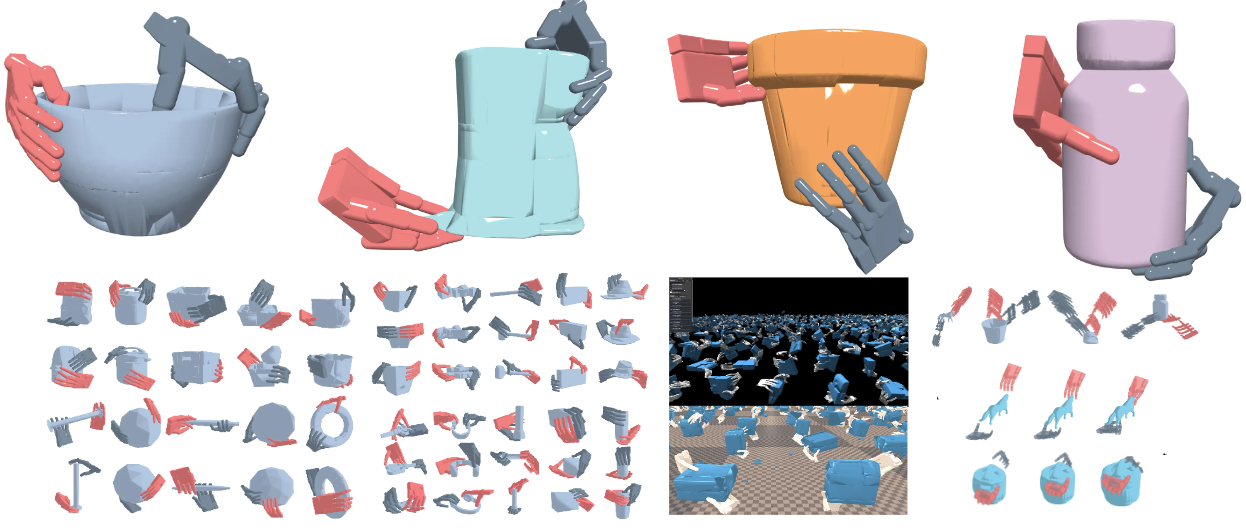
\includegraphics[width=.8\linewidth]{img/BimanGrasp.png}
    \caption{BimanGrasp enables a pair of dexterous hands to grasp various objects, including large and heavy ones, far beyond the capability of unimanual grasping.}
\end{figure*}

\begin{figure*}[htpb]
    \centering
    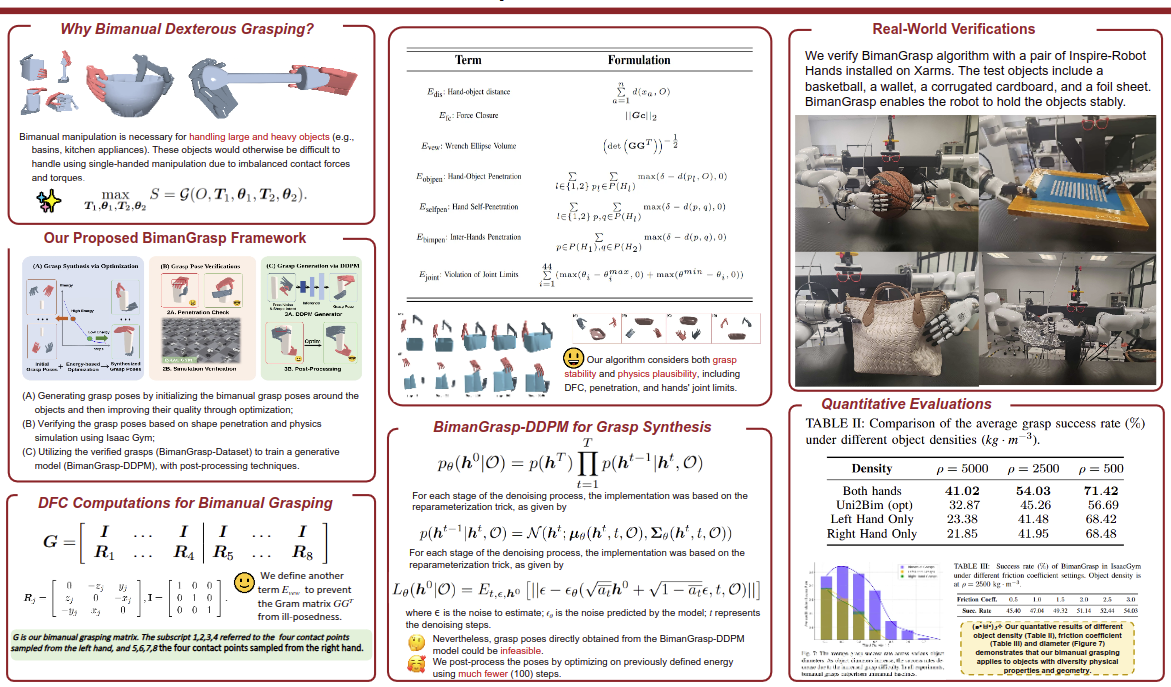
\includegraphics[width=.8\linewidth]{img/bimangrasp_poster.png}
    \caption{BimanGrasp combines differentiable force closure, validation in Isaac Gym, and large-scale data generation for bimanual dexterous grasping.}
\end{figure*}

\newpage

\begin{twocolentry}{
\textit{ }    
    
\textit{ }}
\textbf{SynPolDex}\xspace
    
    \textit{Project at ShanghaiTech RIM Lab and Shanghai AI Lab IPEC. SynPolDex introduces bi-level policy learning for finger-role planning and low-level coordination in multi-fingered robot hands.}

    \textit{ }
\end{twocolentry}

\begin{figure*}[ht]
    \centering
    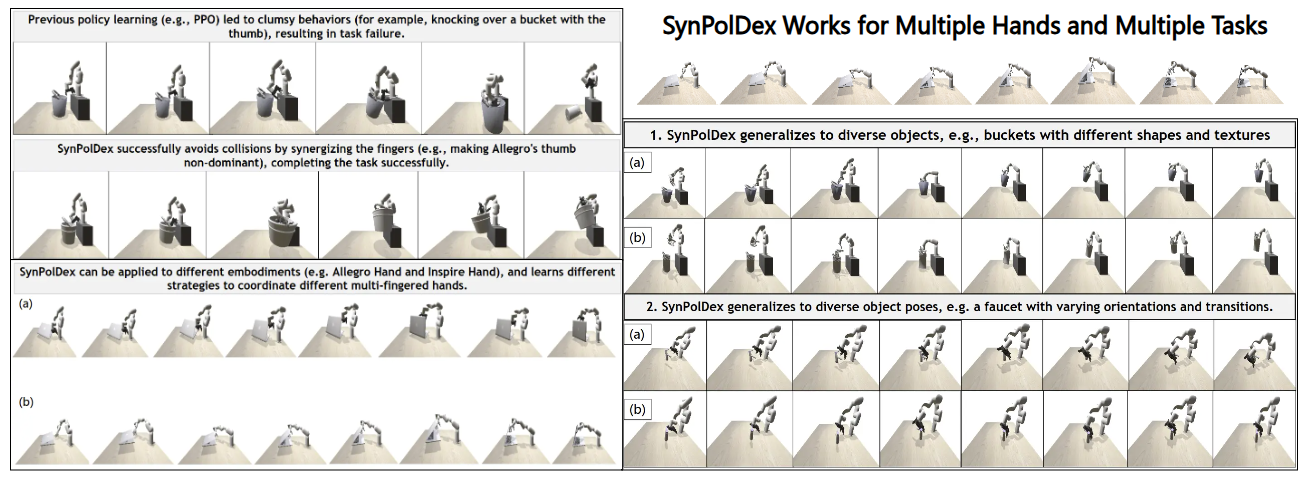
\includegraphics[width=\linewidth]{img/SynPolDex.png}
    \caption{SynPolDex enables object-level and pose-level generalization, can be applied to various hands to accomplish various tasks.}
\end{figure*}

\begin{figure*}[ht]
    \centering
    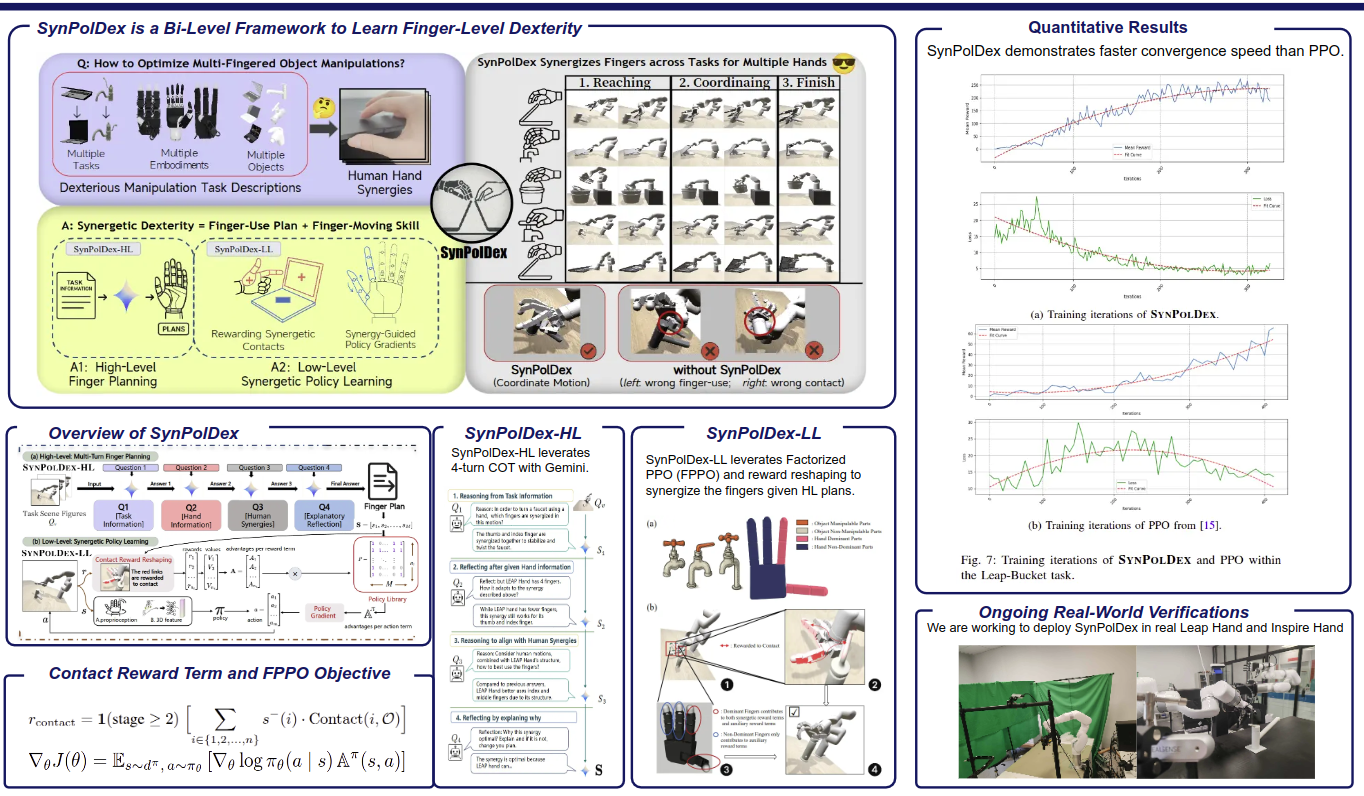
\includegraphics[width=.8\linewidth]{img/SynPolDex-Poster.png}
    \caption{SynPolDex is a Bi-Level framework, including 1) high-level policy, a VLM chain-of-thought to derive a finger-use plan; 2) low-level policy, a factored PPO based reinforcement learning to execute the finger-use plan.}
\end{figure*}

\newpage

\vspace{0.2 cm}

\begin{twocolentry}{
\textit{}    
    
\textit{ }}
\textbf{CleverGrasp}\xspace
    
    \textit{Project at ShanghaiTech RIM Lab. CleverGrasp combines differentiable force closure with finger-level planning, using semantic finger priors to initialize dexterous grasp optimization.}

    \textit{ }
\end{twocolentry}

\begin{figure*}[ht]
    \centering
    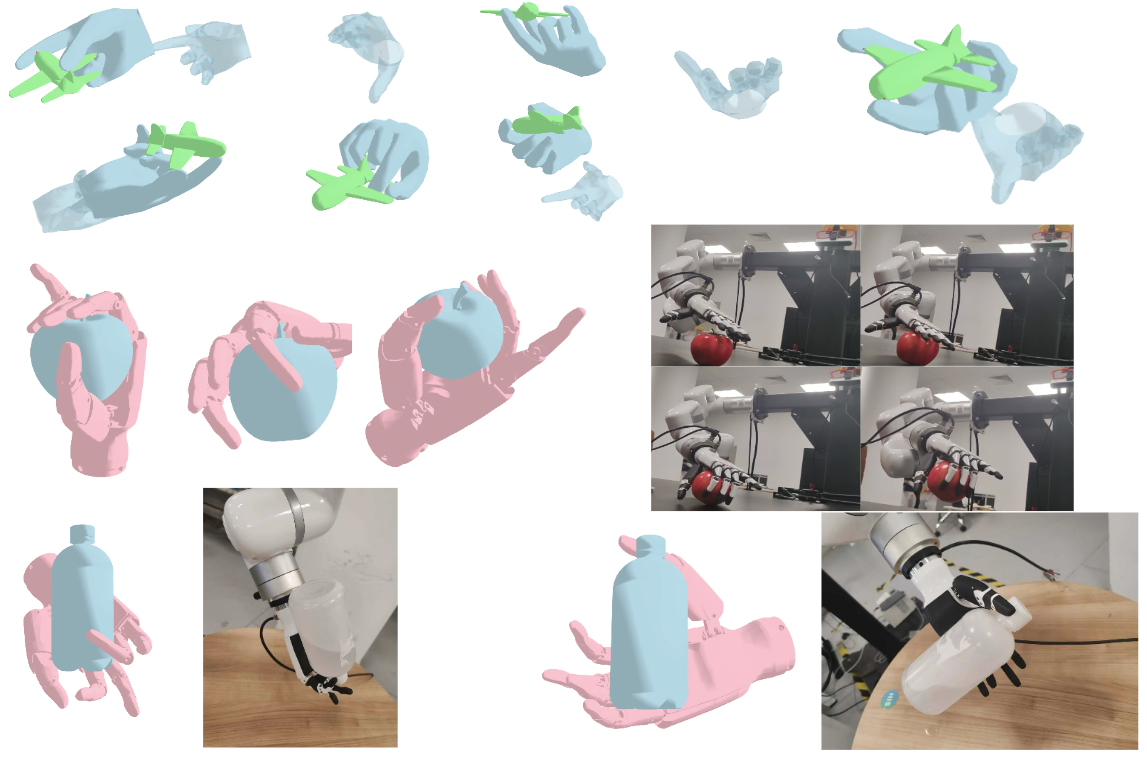
\includegraphics[width=.8\linewidth]{img/clever_grasp.png}
    \caption{CleverGrasp works for both simulation and real world, can grasp various objects in an effortless manner.}
\end{figure*}

\section{SELECTED DEMOS}

\begin{onecolentry}
Recent demo snapshots from dexterous teleoperation and simulation. Full video: \hrefWithoutArrow{https://tsunami-kun.github.io/demo/demo.mp4}{online demo}
\end{onecolentry}

\begin{figure*}[ht]
    \centering
    \begin{minipage}[t]{0.6\linewidth}
        \centering
        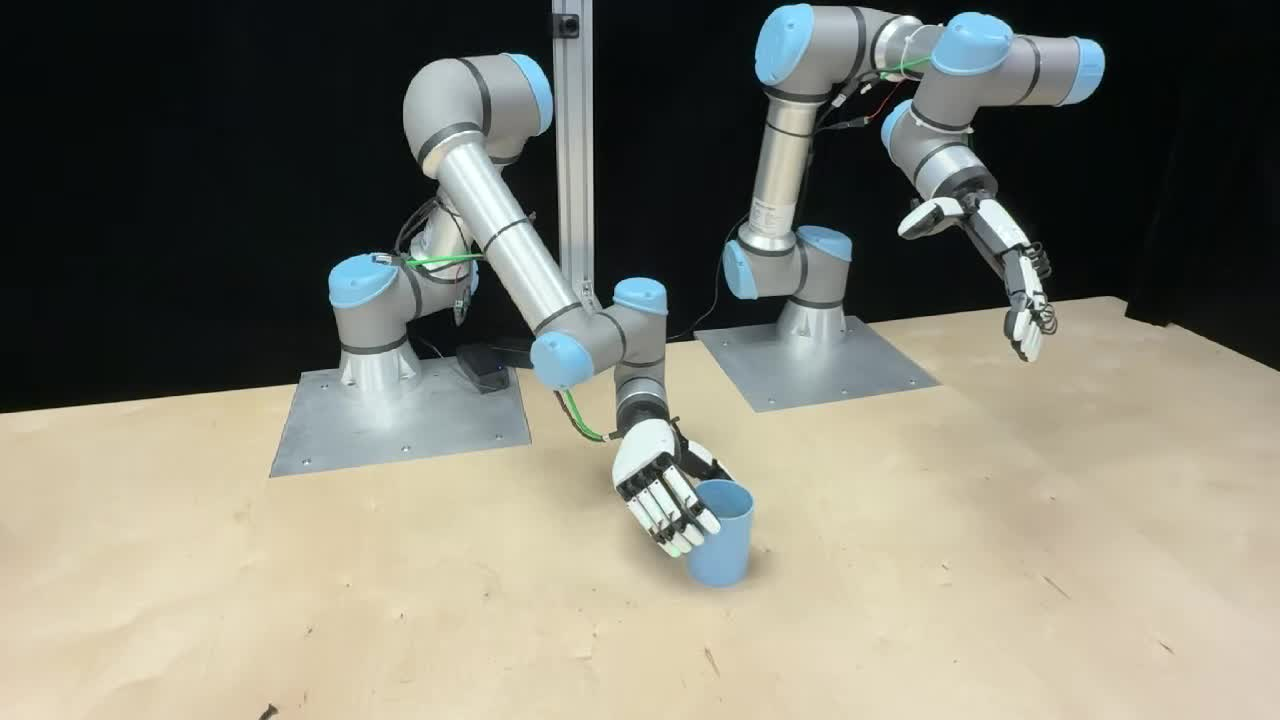
\includegraphics[width=\linewidth]{demo_image/demo_frame.jpg}
    \end{minipage}
    \hfill
    \begin{minipage}[t]{0.32\linewidth}
        \centering
        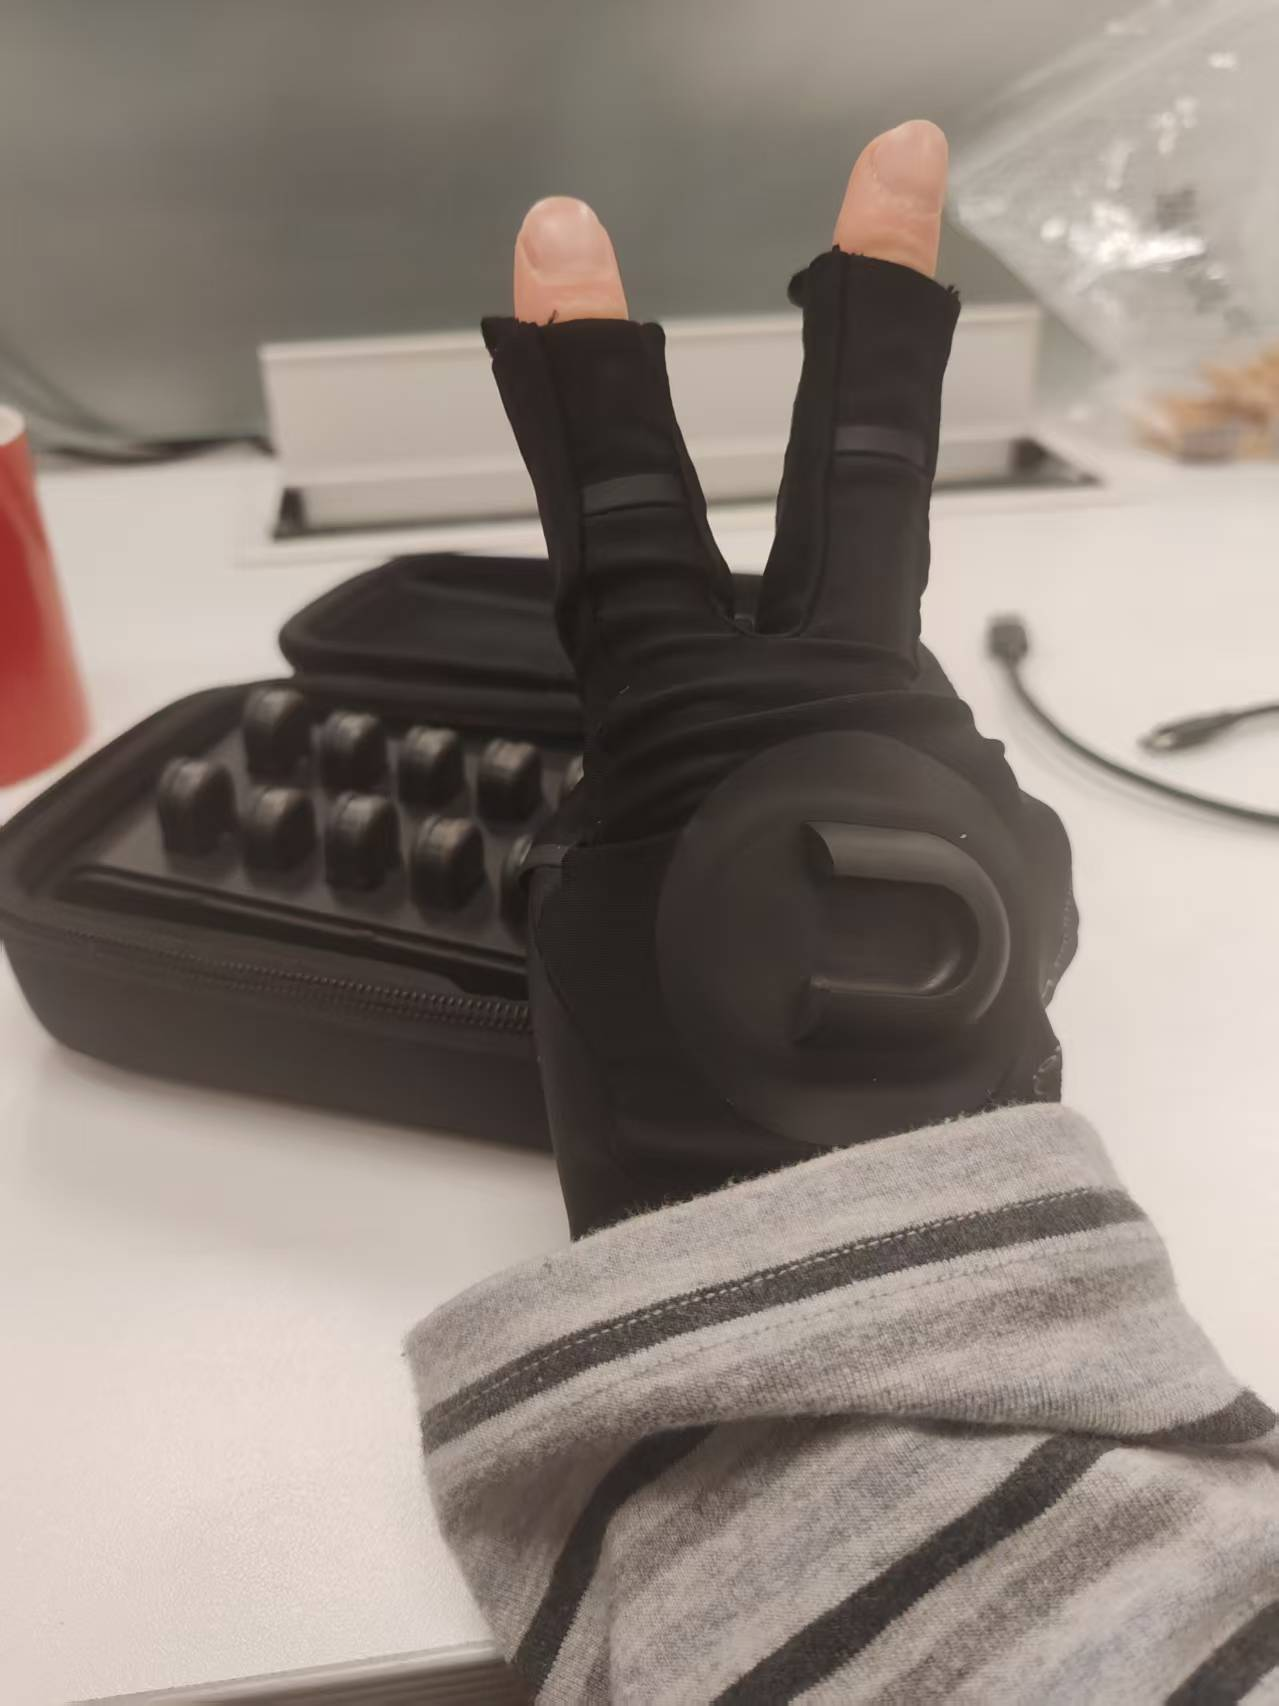
\includegraphics[width=\linewidth]{demo_image/noitum_glove.jpg}
    \end{minipage}
    \caption{Left: a representative frame from the dexterous manipulation demo video. Right: the Noitom glove setup used for teleoperation and data collection.}
    \label{fig:selected-demos}
\end{figure*}

\section{TALKS \& PRESENTATIONS}

\begin{twocolentry}{
\textit{}

\textit{May 2025 (on-line)}}
    \textbf{IEEE International Conference on Robotics and Automation (ICRA)}

    \textit{Bimanual Grasp Synthesis for Dexterous Robot Hands}
\end{twocolentry}

\vspace{0.15 cm}

\begin{twocolentry}{
\textit{}

\textit{Dec 2024}}
    \textbf{ShanghaiTech SI100B: Introduction to Information Science (TA Lecture)}

    \textit{Object Oriented Programming, Git, and Introduction to Game Development}
\end{twocolentry}

\section{TEACHING EXPERIENCES}

\begin{itemize}
    \item Teaching Assistant, Embodied Intelligence (ShanghaiTech University, 2025 Spring; course instructor: Jiayuan Gu)
    \item Teaching Assistant, Introduction to Information Science (ShanghaiTech University, 2024 Fall; course instructor: Kewei Tu)
\end{itemize}

\section{SERVICES}

\begin{itemize}
    \item Reviewer, IEEE Robotics and Automation Letters (RA-L)
    \item Reviewer, IEEE/ASME Transactions on Mechatronics
    \item Reviewer, The 64rd IEEE Conference on Decision and Control (CDC 2025)
    \item Reviewer, 2025 IEEE-RAS 24th International Conference on Humanoid Robots (Humanoids 2025)
\end{itemize}

\section{OPEN SOURCE}

\begin{itemize}
    \item Maintainer, \hrefWithoutArrow{https://github.com/Tsunami-kun/awesome-humanoid-manipulation}{Awesome Humanoid Manipulation} (100+ GitHub stars), a curated map of human-like manipulation, dexterous grasping, and humanoid research directions.
\end{itemize}

\section{SELECTED COURSE PROJECTS}

\begin{twocolentry}{
\textit{}    
    
\textit{2023 Fall (Mobile Manipulation Course, A)}}
\textbf{KiwiPicker}\xspace
    
    \textit{Using a complete robotic system (AgileX Bunker + CR5 Arm + LiDAR + 2 RealSense D435 Cameras + Parallel Gripper), we implemented a full pipeline integrating navigation, object recognition, grasp detection, and robotic arm control. }

    \textit{ }
\end{twocolentry}

\begin{figure*}[ht]
    \centering
    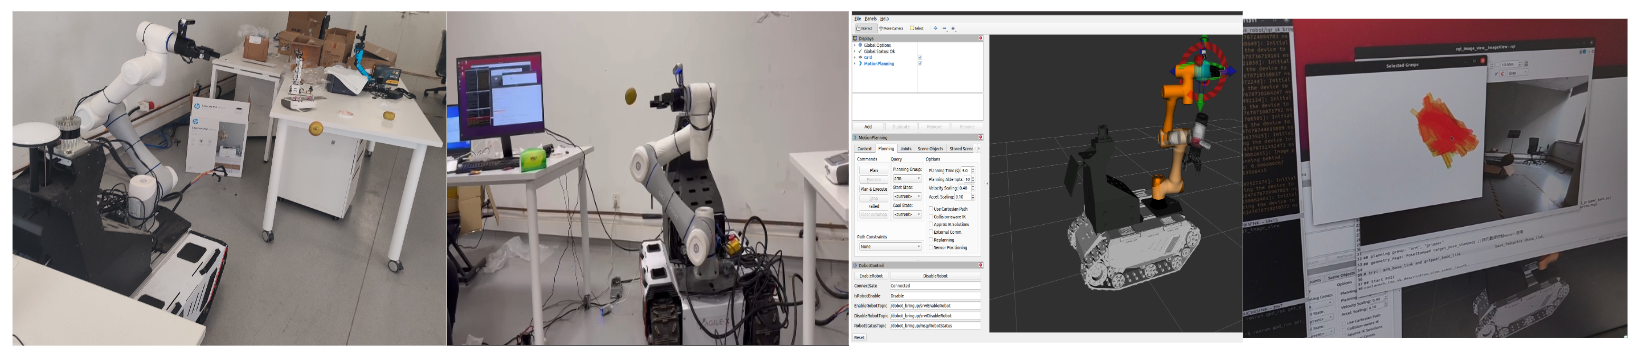
\includegraphics[width=\linewidth]{img/kiwi_moma.png}
    \caption{KiwiPicker leveraged Robotic Operating System (ROS) and Grasp Pose Detection (GPD) to grasp kiwifruit models in real environments.}
\end{figure*}



\newpage
    
\vspace{0.2 cm}

\begin{twocolentry}{
\textit{}    


\textit{2024 Spring (Intro to Algebraic Geometry, A)}}
\textbf{Obstructions in Geometric Complexity Theory}\xspace
    
    \textit{In this project, I conducted a literature view on the newest advancement in geometric complexity theory. Specfically, I surveyed obstruction method, which is a promising way to answer if $\mathsf{VP} \neq \mathsf{VNP}$, which is the geometric analogy of the famous $\mathsf{P} \neq \mathsf{NP}$ problem.}

    \textit{}
\end{twocolentry}



\section{ROBOT FRIENDS}

\textbf{Robots I actively worked with during my projects:}

\begin{itemize}
    \item Inspire Dexterous Hands RH56DFTP
    \item Leap Dexterous Hand
    \item Robot arms (X-Arm, Dobot CR-5, UR10 Arm) 
    \item AgileX Bucket
\end{itemize}


\begin{figure*}[ht]
    \centering
    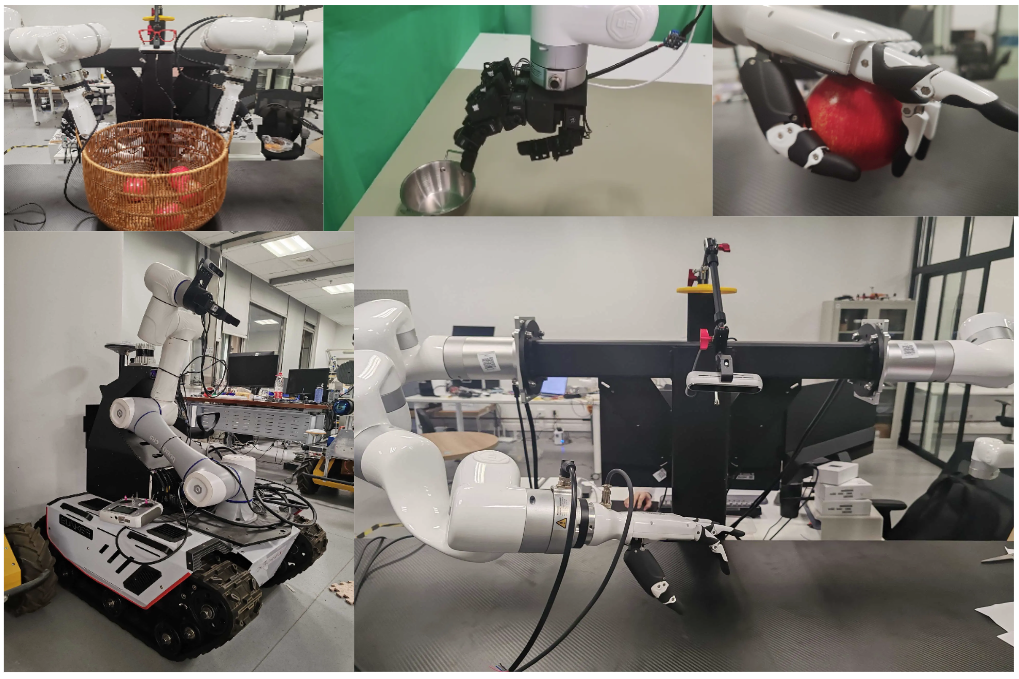
\includegraphics[width=\linewidth]{img/robot_friends_a.png}
    \caption{Robot friends I frequently work with.}
\end{figure*}

\vspace{0.2 cm}



\textbf{Robots I once played with:}

\begin{itemize}
    \item Inspire Dexterous Hands RH56DFX
    \item 16 DoF Leap Hand
    \item 4-Fingered Hydraulic Exoskeleton
    \item Fourier GR1 Humanoid Robot
    \item Flexiv RIZON 4 Arm
    \item Fast-UMI Data Collection Gripper
\end{itemize}

\begin{figure*}[ht]
    \centering
    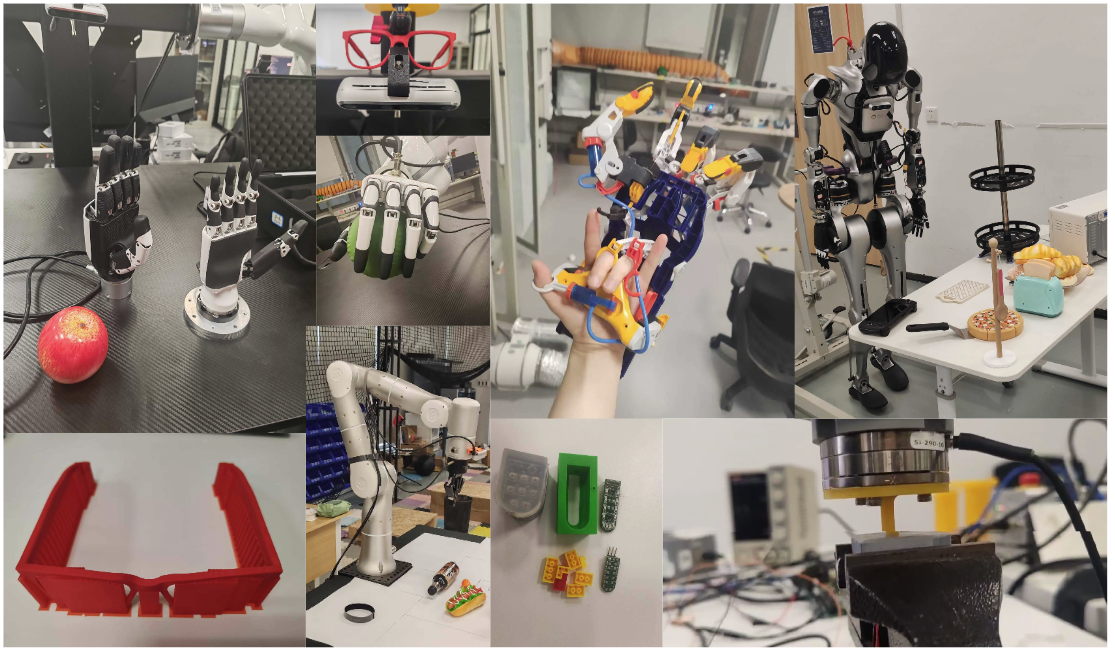
\includegraphics[width=\linewidth]{img/robot_friends_b.png}
    \caption{Robot friends I once worked with.}
\end{figure*}

\section{HONORS}

\textbf{Graduate}

\begin{itemize}
    \item ShanghaiTech University Merit Student (2024-2025)
\end{itemize}

\textbf{Undergraduate}

\begin{itemize}
    \item Merit Person and Leader of 3rd Prize Group. Topic: Autonomous Driving Industry (2020)
\end{itemize}

\section{ACTIVITIES}

\begin{itemize}
    \item 1st in ShanghaiTech University Industry Research Competition (2025, Teammate: Hao Wei, Heng Liu). Report title: \emph{The Future of Humanoid Robots}. 


\begin{figure*}[ht]
    \centering
    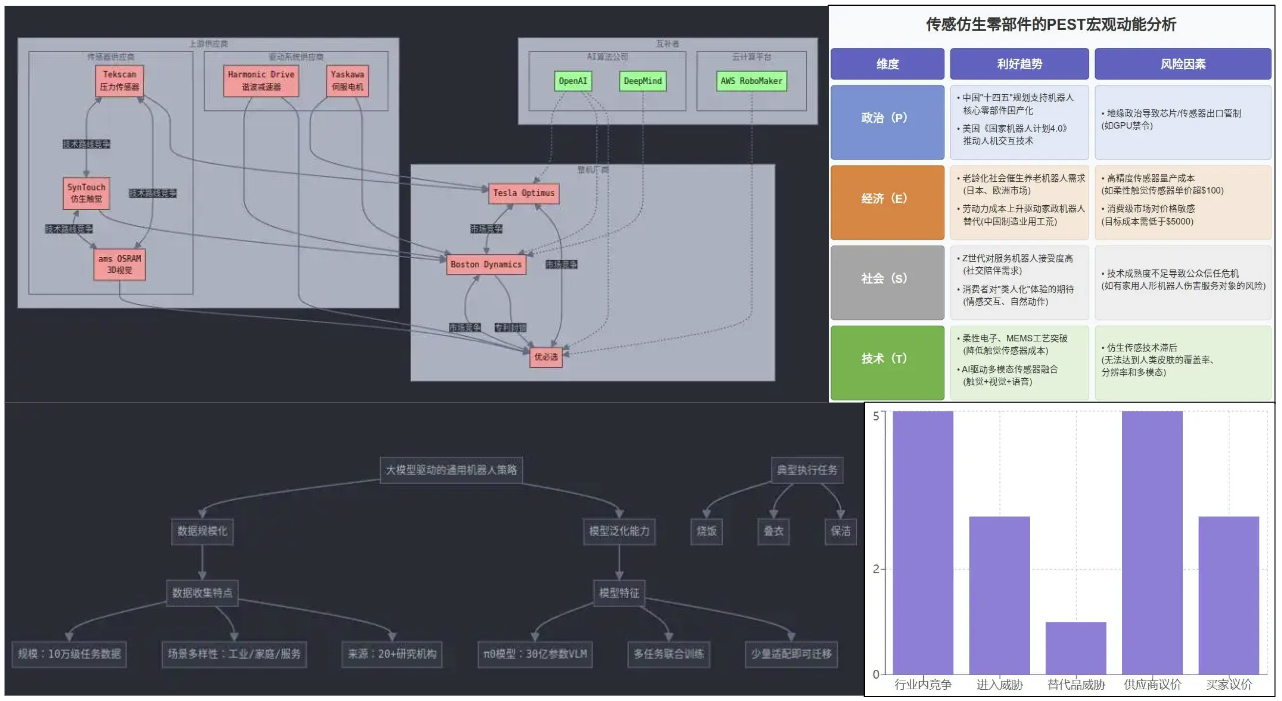
\includegraphics[width=.8\linewidth]{img/humanoid_report.png}
    \caption{We conducted various industrial analysis on humanoid robotics during the Competition.}
\end{figure*}


    \item Certificate for Future Sensing Sci-Art Workshop (2025, Teammate: Sijie Xu, Jingtong Zhang, Jichen Zhou). Piece title: \emph{Beyond the pulse: There is no bot}.


\begin{figure*}[ht]
    \centering
    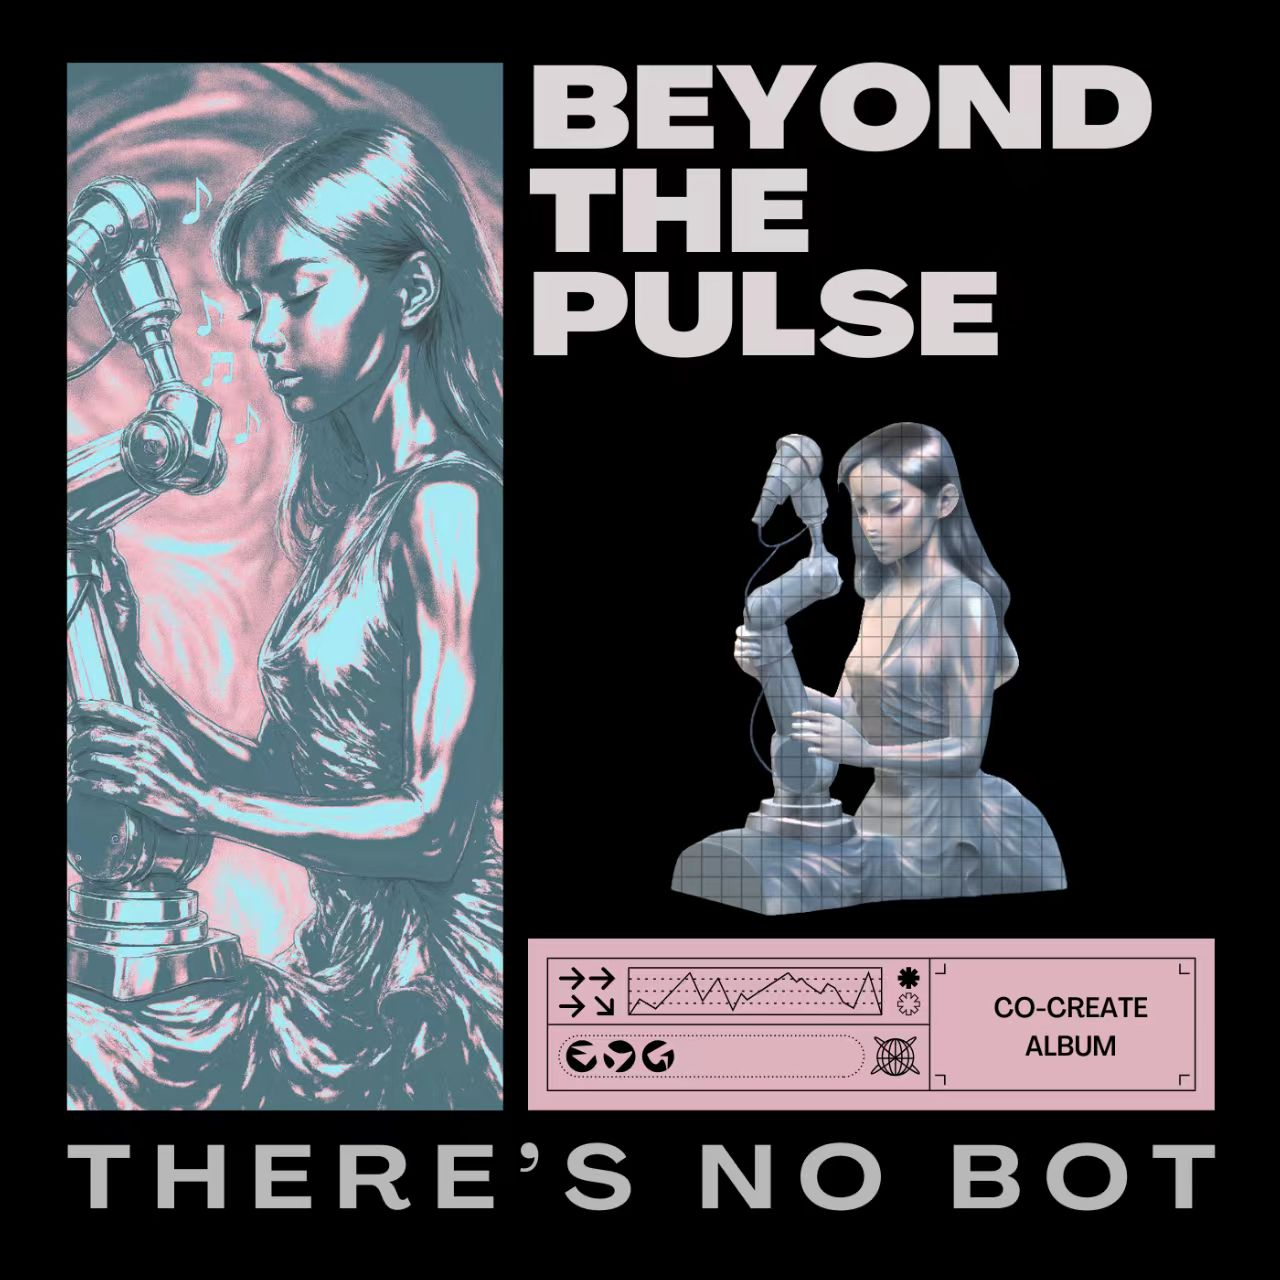
\includegraphics[width=.7\linewidth]{img/no_bot.jpg}
    \caption{\emph{Beyond the pulse: There is no bot} combines music generation and robotic arm motion. One performer moves the arm, and music are produced by mapping the joint angles to different chords based on music theory.}
\end{figure*}
    


\end{itemize}


\end{document}
